\documentclass[12pt]{article}

\usepackage[letterpaper, margin=1in]{geometry}
\usepackage{tikz}
\usetikzlibrary{calc}
\usepackage{enumitem}
\usepackage{graphicx}
\usepackage{hyperref} % Add this package for hyperlinks
\pdfminorversion=7 % Allow inclusion of PDF version 1.7 files

\setlength{\parskip}{1em}
\setlength{\parindent}{0pt}

\begin{document}

\begin{titlepage}
    \centering
    \vfill
    \vspace*{2.5in}
    \begin{tikzpicture}[remember picture, overlay]
        \draw [line width=1pt, rounded corners=10pt] 
            ($(current page.north west) + (0.5in,-0.5in)$) rectangle 
            ($(current page.south east) + (-0.5in,0.5in)$);
    \end{tikzpicture}
    {\Huge\bfseries Capstone 2025 - Initial Proposal \par}
    \vspace{0.2in}
    {\LARGE Tolly Zhang \par}    
    \vspace{0.2in}
    {\LARGE December 20, 2024 \par}
    \vfill
\end{titlepage}

\newpage
\section{Project Overview}
\subsection{Objective}
The objective of this project is to develop an aerial package delivery system capable of transporting small to medium-sized payloads over short to medium-range distances. The system will consist of four primary components:
\begin{enumerate}
    \item Dynamic Aerial Mobility System (DAMS)
    \item Payload Retrieval and Deployment Module (PRDM)
    \item Automated Flight Navigation System (AFNS)
    \item Adaptive Flight Control Interface (AFCI)
\end{enumerate}

\subsection{Key Performance Indicators (KPIs)}
The success of the project will be measured using the following key performance indicators:
\begin{itemize}
    \item Drop-off accuracy (i.e., distance from the intended delivery location).
    \item Mission success rate (i.e., the ratio between the number of successful missions and the total number of attempted missions).
    \item Average distance traveled per unit of battery capacity (km//wh).
    \item Maximum operational time per full charge under normal conditions.
    \item Time and energy required to switch between VTOL and fixed-wing modes.
    \item Maximum payload weight the system can transport reliably.
    \item Maximum allowed deviation from center of gravity during flight with varying payload distributions.
    \item Time required to autonomously and reliably pick up or drop off a payload.
    \item Percentage of successful obstacle detections and avoidances during flight.
    \item Time reduced in delays for simultaneous delivery missions.
    \item Average time latency for the Adaptive Flight Control Interface (AFCI) to execute commands.
    \item Time required for an operator to prepare and verify a device for flight.
    \item User satisfaction scores on a scale of 1-10 based on ease of use and reliability.
    \item Percentage of successful landings after a simulated single/multi-motor or system failure.
    \item Performance under various weather conditions.
    \item Percentage of correctly identified and reported system errors.
    \item Average total cost of operation per single delivery.
    \item Average time between required repairs or system maintenance tasks.
\end{itemize}

\subsection{Timeline}
Forenote: The project is \textit{not} expected to be completed by the Capstone presentation in September 2025. The timeline below outlines the key milestones for the project:
\begin{itemize}
    \item \textbf{January–February 2025}:
    \begin{itemize}
        \item Research, ideation, and initial concept development.
        \item Prototyping of different systems in the DAMS and PRDM.
    \end{itemize}
    \item \textbf{March–June 2025}:
    \begin{itemize}
        \item Component selection for the DAMS and PRDM.
        \item CAD development and simulation of the system architecture.
    \end{itemize}
    \item \textbf{July 2025}:
    \begin{itemize}
        \item Manufacturing and assembly of the designed components.
        \item Initial testing of individual components and subsystems.
    \end{itemize}
    \item \textbf{August–September 2025}:
    \begin{itemize}
        \item Integration of the components, testing, and initial flight trials.
    \end{itemize}
    \item \textbf{October–December 2025}:
    \begin{itemize}
        \item Refinement of DAMS and PRDM.
        \item Development of the AFNS and AFCI.
    \end{itemize}
\end{itemize}

\newpage
\section{Concept Development}
\subsection{System Architecture}

\subsubsection{Dynamic Aerial Mobility System (DAMS)}
The DAMS will feature a Vertical Take-Off and Landing (VTOL) flight system, capable of switching between VTOL and fixed-wing flight modes. The VTOL mode will be used for takeoff and landing, while the fixed-wing mode will facilitate efficient cruising. The DAMS integrates the \textbf{Dynamic Flight Control Unit}, which ensures smooth transitions between flight modes using \textbf{actuators} to control components such as rudders, elevators, and ailerons. Sensors, including IMUs (Inertial Measurement Units) and LIDAR, will provide real-time feedback for stability and maneuverability during flight. The DAMS will also interface with the \textbf{Automated Flight Navigation System (AFNS)} for autonomous flight control.

\subsubsection{Payload Retrieval and Deployment Module (PRDM)}
The PRDM will be responsible for the autonomous retrieval and deployment of payloads. It will utilize the \textbf{Payload Control Unit} to manage and control various components for payload operations. Key features will include:
\begin{itemize}
    \item An opening/closing door for payload access, controlled by actuators.
    \item A clamp mechanism to securely hold the payload during flight.
    \item A winch mechanism for raising and lowering the payload during retrieval and deployment.
    \item Proximity and weight sensors to monitor payload positioning and distribution, providing real-time data to the DAMS to ensure stability and balance.
\end{itemize}
The PRDM will work in coordination with the \textbf{DAMS} to ensure the aircraft maintains stability and efficient operation during payload operations.

\subsubsection{Automated Flight Navigation System (AFNS)}
The AFNS will determine the optimal flight path from the source to the destination, leveraging data from onboard sensors such as GPS, cameras, and LIDAR. It will provide precise navigational instructions to the DAMS and coordinate with other onboard systems for efficient path planning. The AFNS will also support multi-aircraft management, enabling the simultaneous coordination of multiple deliveries and flight routes.

\subsubsection{Adaptive Flight Control Interface (AFCI)}
The AFCI will serve as the human-machine interface, allowing the operator to interact with both the AFNS and the DAMS. It will feature:
\begin{itemize}
    \item Multiple modes of operation, including manual, semi-autonomous, and autonomous.
    \item Input devices such as screens, keyboards, mice, and controllers.
    \item A speech control interface for hands-free operation, integrated with an audio recorder and speaker system.
    \item A heads-up display (HUD) for providing real-time telemetry and flight data to the operator.
\end{itemize}
The AFCI will ensure that operators have full control and oversight during all phases of operation, while enabling user-friendly interaction with the system.

\noindent\rule{\textwidth}{0.4pt}

Below is a diagram displaying the correlations between the four different components (created using \href{https://www.diagrams.net/}{diagrams.net}):

\begin{figure}[h]
    \centering
    \begin{tikzpicture}
        \node[inner sep=0pt] (diagram) at (0,0) {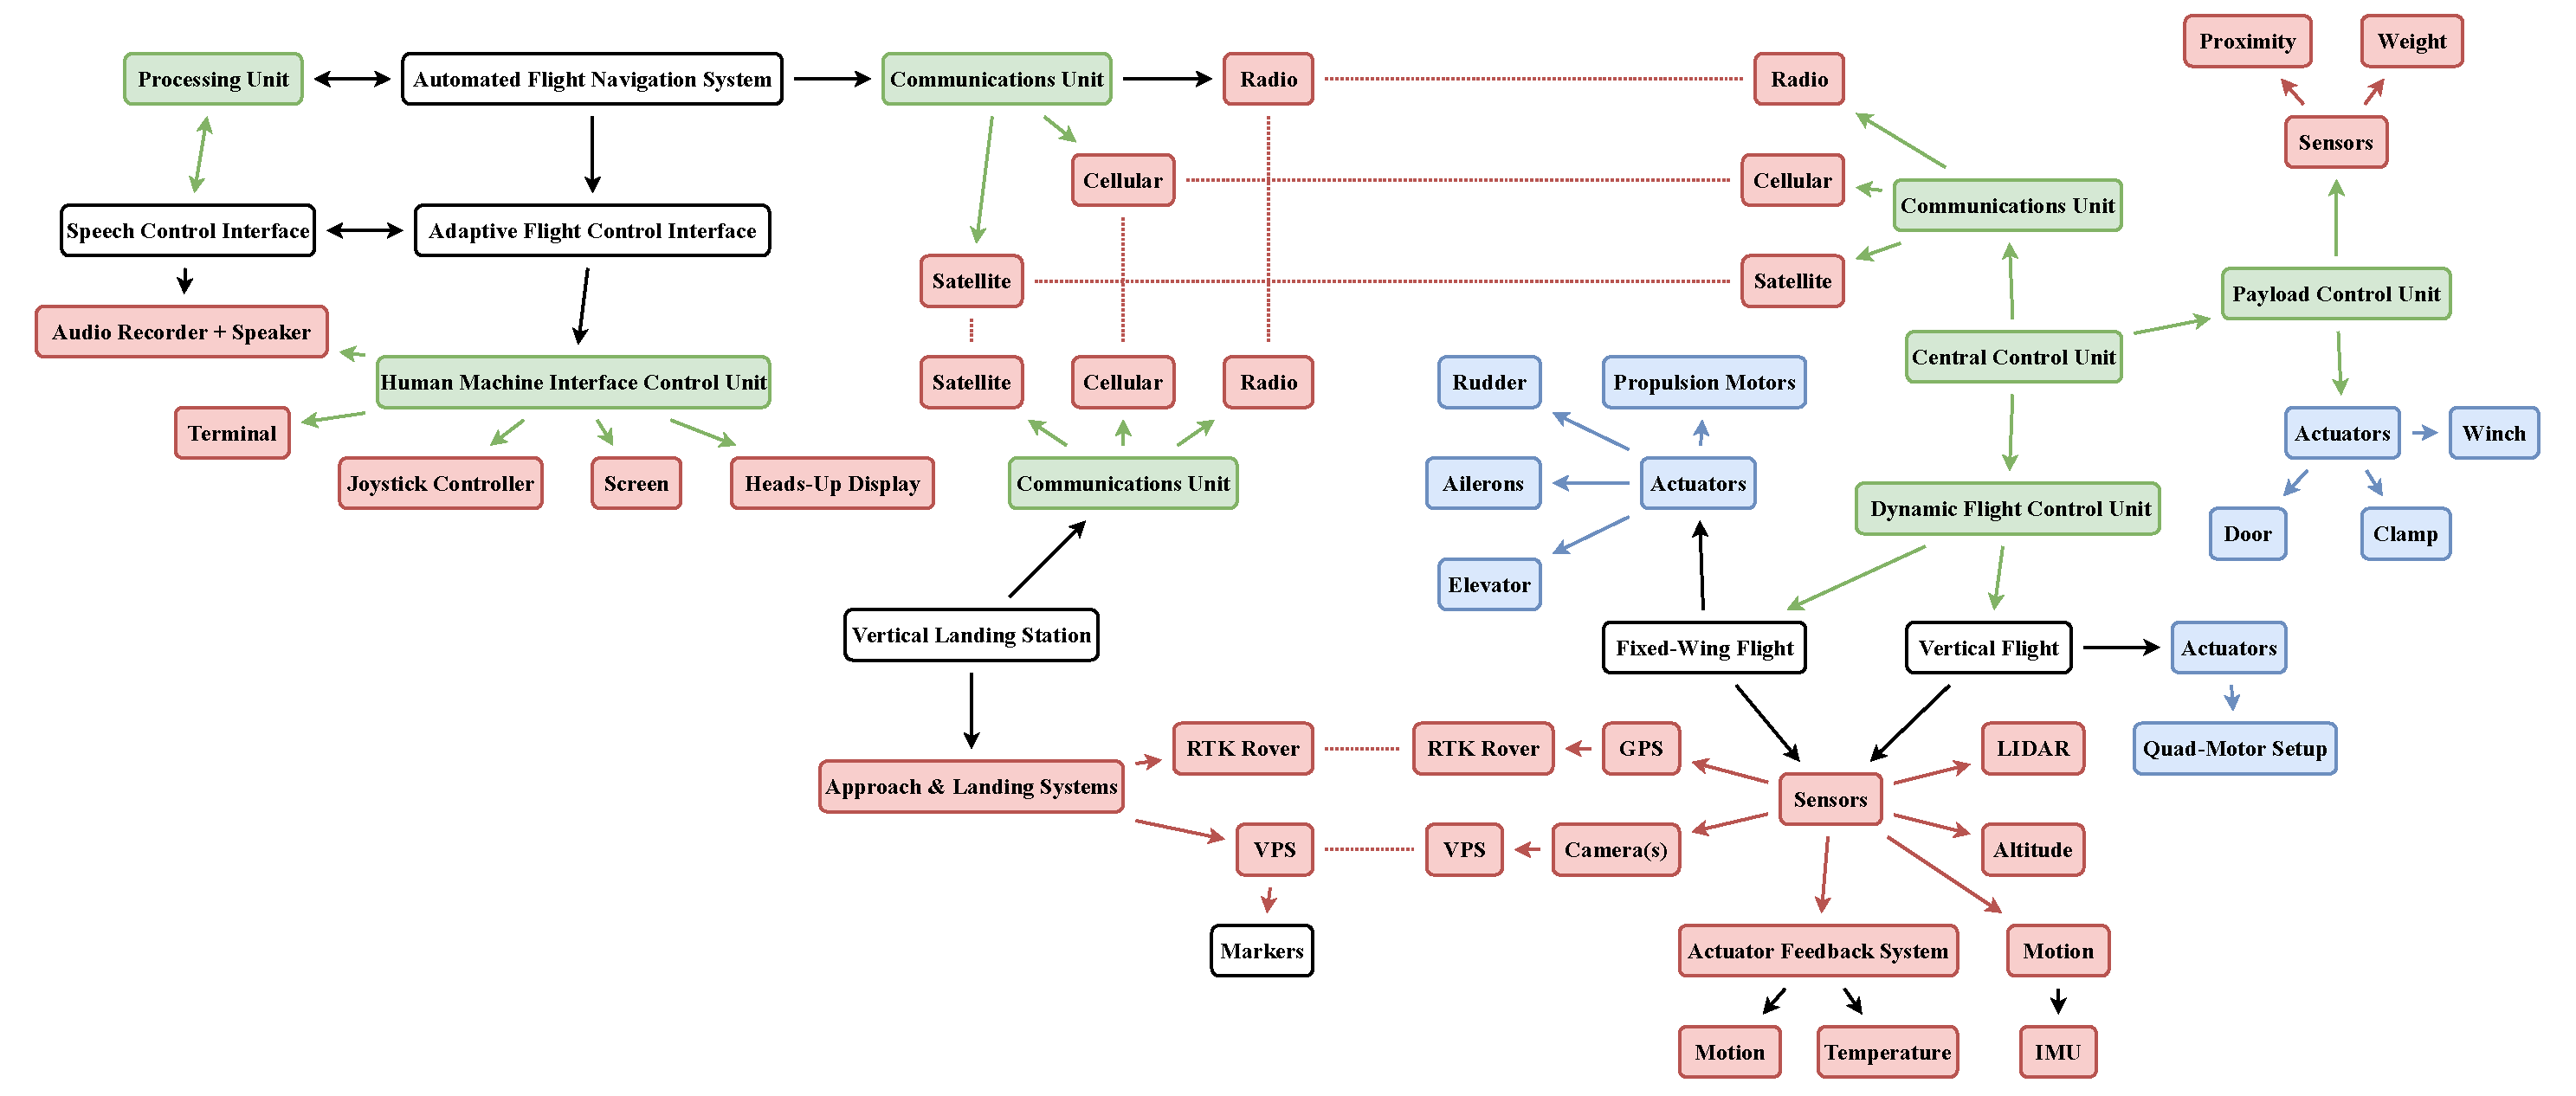
\includegraphics[width=\textwidth]{resources/system-architecture.drawio.pdf}};
        \draw [line width=1pt, rounded corners=10pt] 
            (diagram.north west) rectangle 
            (diagram.south east);
    \end{tikzpicture}
    \caption{System Architecture Diagram}
\end{figure}

\end{document}
